\documentclass[hidelinks,a4paper,11pt, nofootinbib]{article}
\usepackage[left=2.5cm,right=2.5cm,top=4cm,bottom=3.5cm]{geometry}
\usepackage[spanish, es-tabla]{babel} %es-tabla es para que ponga Tabla en vez de Cuadro en el caption
\usepackage[utf8]{inputenc}
\usepackage[T1]{fontenc}
\usepackage{xspace}
\usepackage{xargs}
\usepackage{fancyhdr}
\usepackage{lastpage}
\usepackage{caratula}
\usepackage{enumitem} %Permite modificar los margenes de lsa listas
\usepackage[bottom]{footmisc}
\usepackage{amsmath}
\usepackage{amssymb}
\usepackage{algorithm}
\usepackage[noend]{algpseudocode}
\usepackage{array}
\usepackage{xcolor,colortbl}
\usepackage{amsthm}
\usepackage{listings}
\usepackage{soul}
\usepackage{graphicx}
\usepackage{sidecap}
\usepackage{amsmath}
\usepackage{wrapfig}
\usepackage{caption}
\usepackage{mathpazo}
\usepackage{booktabs,tabularx}
\usepackage{ulem}


\setlength{\parindent}{4em}
\setlength{\parskip}{1em}

%Formato de los links
\usepackage{hyperref}
\hypersetup{
  colorlinks   = true, %Colours links instead of ugly boxes
  urlcolor     = blue, %Colour for external hyperlinks
  linkcolor    = blue, %Colour of internal links
  citecolor   = red %Colour of citations
}

\usepackage{comment}
\captionsetup[table]{labelsep=space}


\setlength{\parindent}{4em}
\setlength{\parskip}{0.5em}


%%fancyhdr
\pagestyle{fancy}
\thispagestyle{fancy}
\addtolength{\headheight}{1pt}
\lhead{Bases de Datos}
\rhead{$1º$ cuatrimestre de 2017}
\cfoot{\thepage\ / \pageref{LastPage}}
\renewcommand{\footrulewidth}{0.4pt}
\renewcommand{\labelitemi}{$\bullet$}

%%caratula
\materia{Bases de Datos}
\titulo{Trabajo Práctico Número 2}
\subtitulo{Mundiales de Taekwon Do: Histórico de Competiciones}
\grupo{Grupo 3}
\integrante{Ciruelos Rodríguez, Gonzalo}{063/14}{gonzalo.ciruelos@gmail.com}
\integrante{Ferrante, Alejandro}{371/09}{matapalabras@hotmail}
\integrante{Goldstein, Brian}{027/14}{brai.goldstein@gmail.com}
\integrante{Thibeault, Gabriel}{114/13}{gabriel.eric.thibeault@gmail.com}

% \fecha{24 de Junio de 2016}
\begin{document}

\maketitle

\tableofcontents
\newpage

\section{Introducción}
Este trabajo se basa en modelar un sistema de resultados históricos de Mundiales de Taekwondo usando herramientas de diseño de bases de dato no-relacionales. Además deberemos implementar el sistema en una base de datos NoSQL particular.

Primero necesitamos modelar el problema utilizando un diagrama de entidad--relación. Luego debemos pasar del modelo relacional a un modelo no-relacional. Para eso utilizaremos un diagrama de interacción de documentos, que obtendremos a partir del de entidad--relación.

El diagrama de interacción de documentos podrá ser traducido a un JSON Schema que finalmente se verá plasmado en una implementación física en una base de datos NoSQL concreta.
El motor de base de datos que utilizaremos es \textbf{RethinkDB}.


\newpage

\section{Modelos y Diseño}
\subsection{Diagrama de Entidad--Relación}

\subsubsection{Suposiciones}

\subsubsection{Diagrama}

\newpage

\noindent
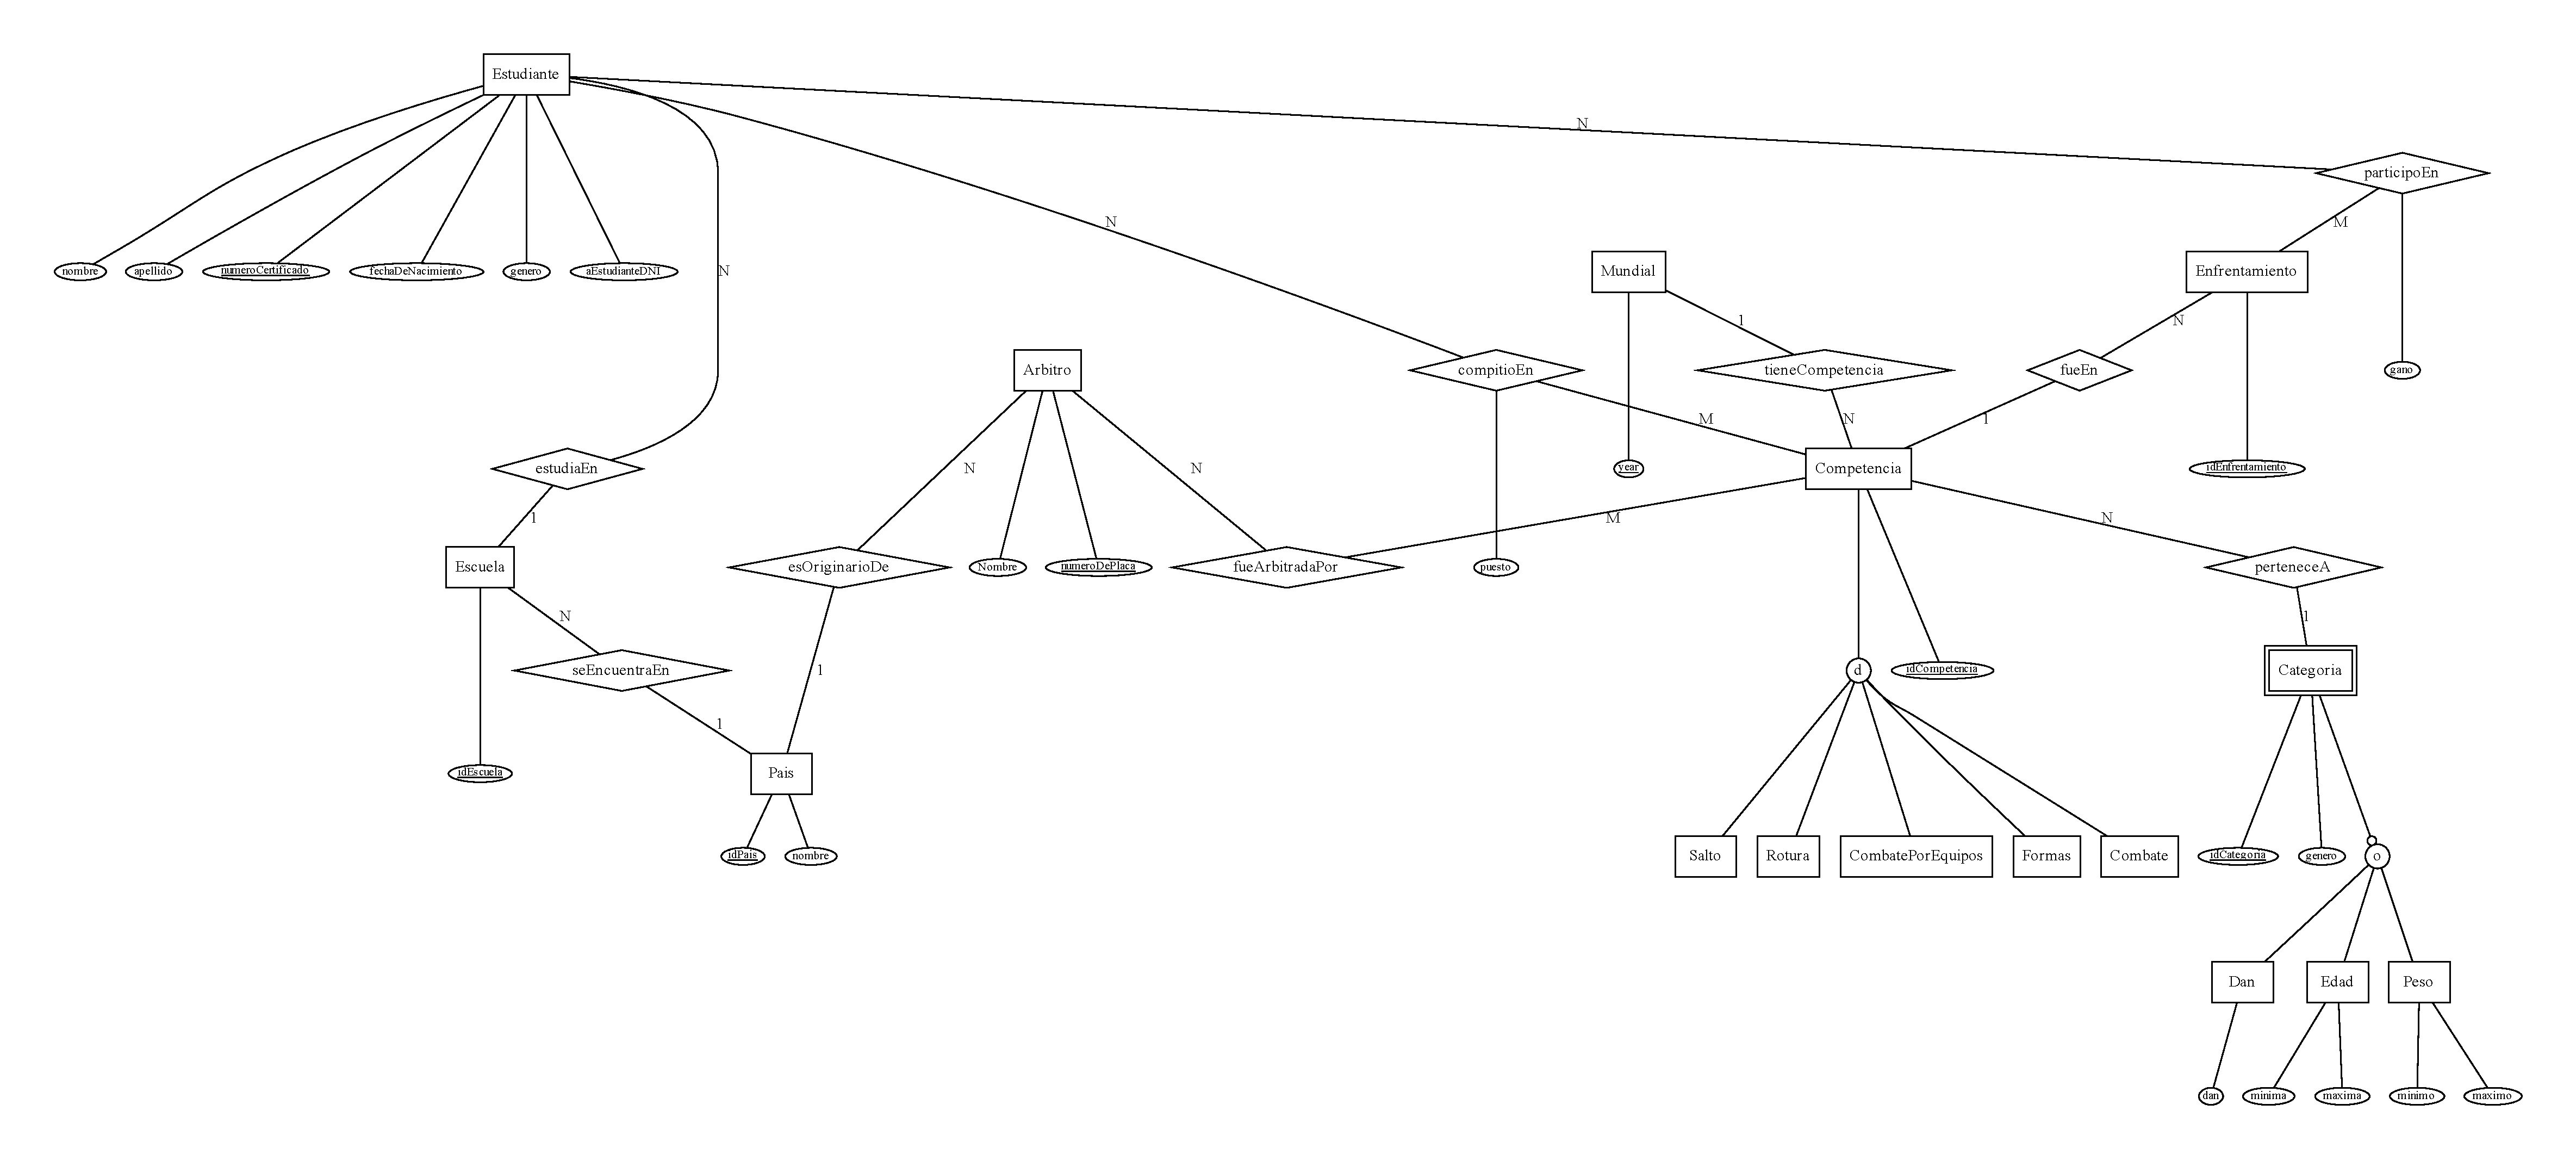
\includegraphics[angle=90,height=23cm]{../mer/mer-dot.pdf}

\noindent
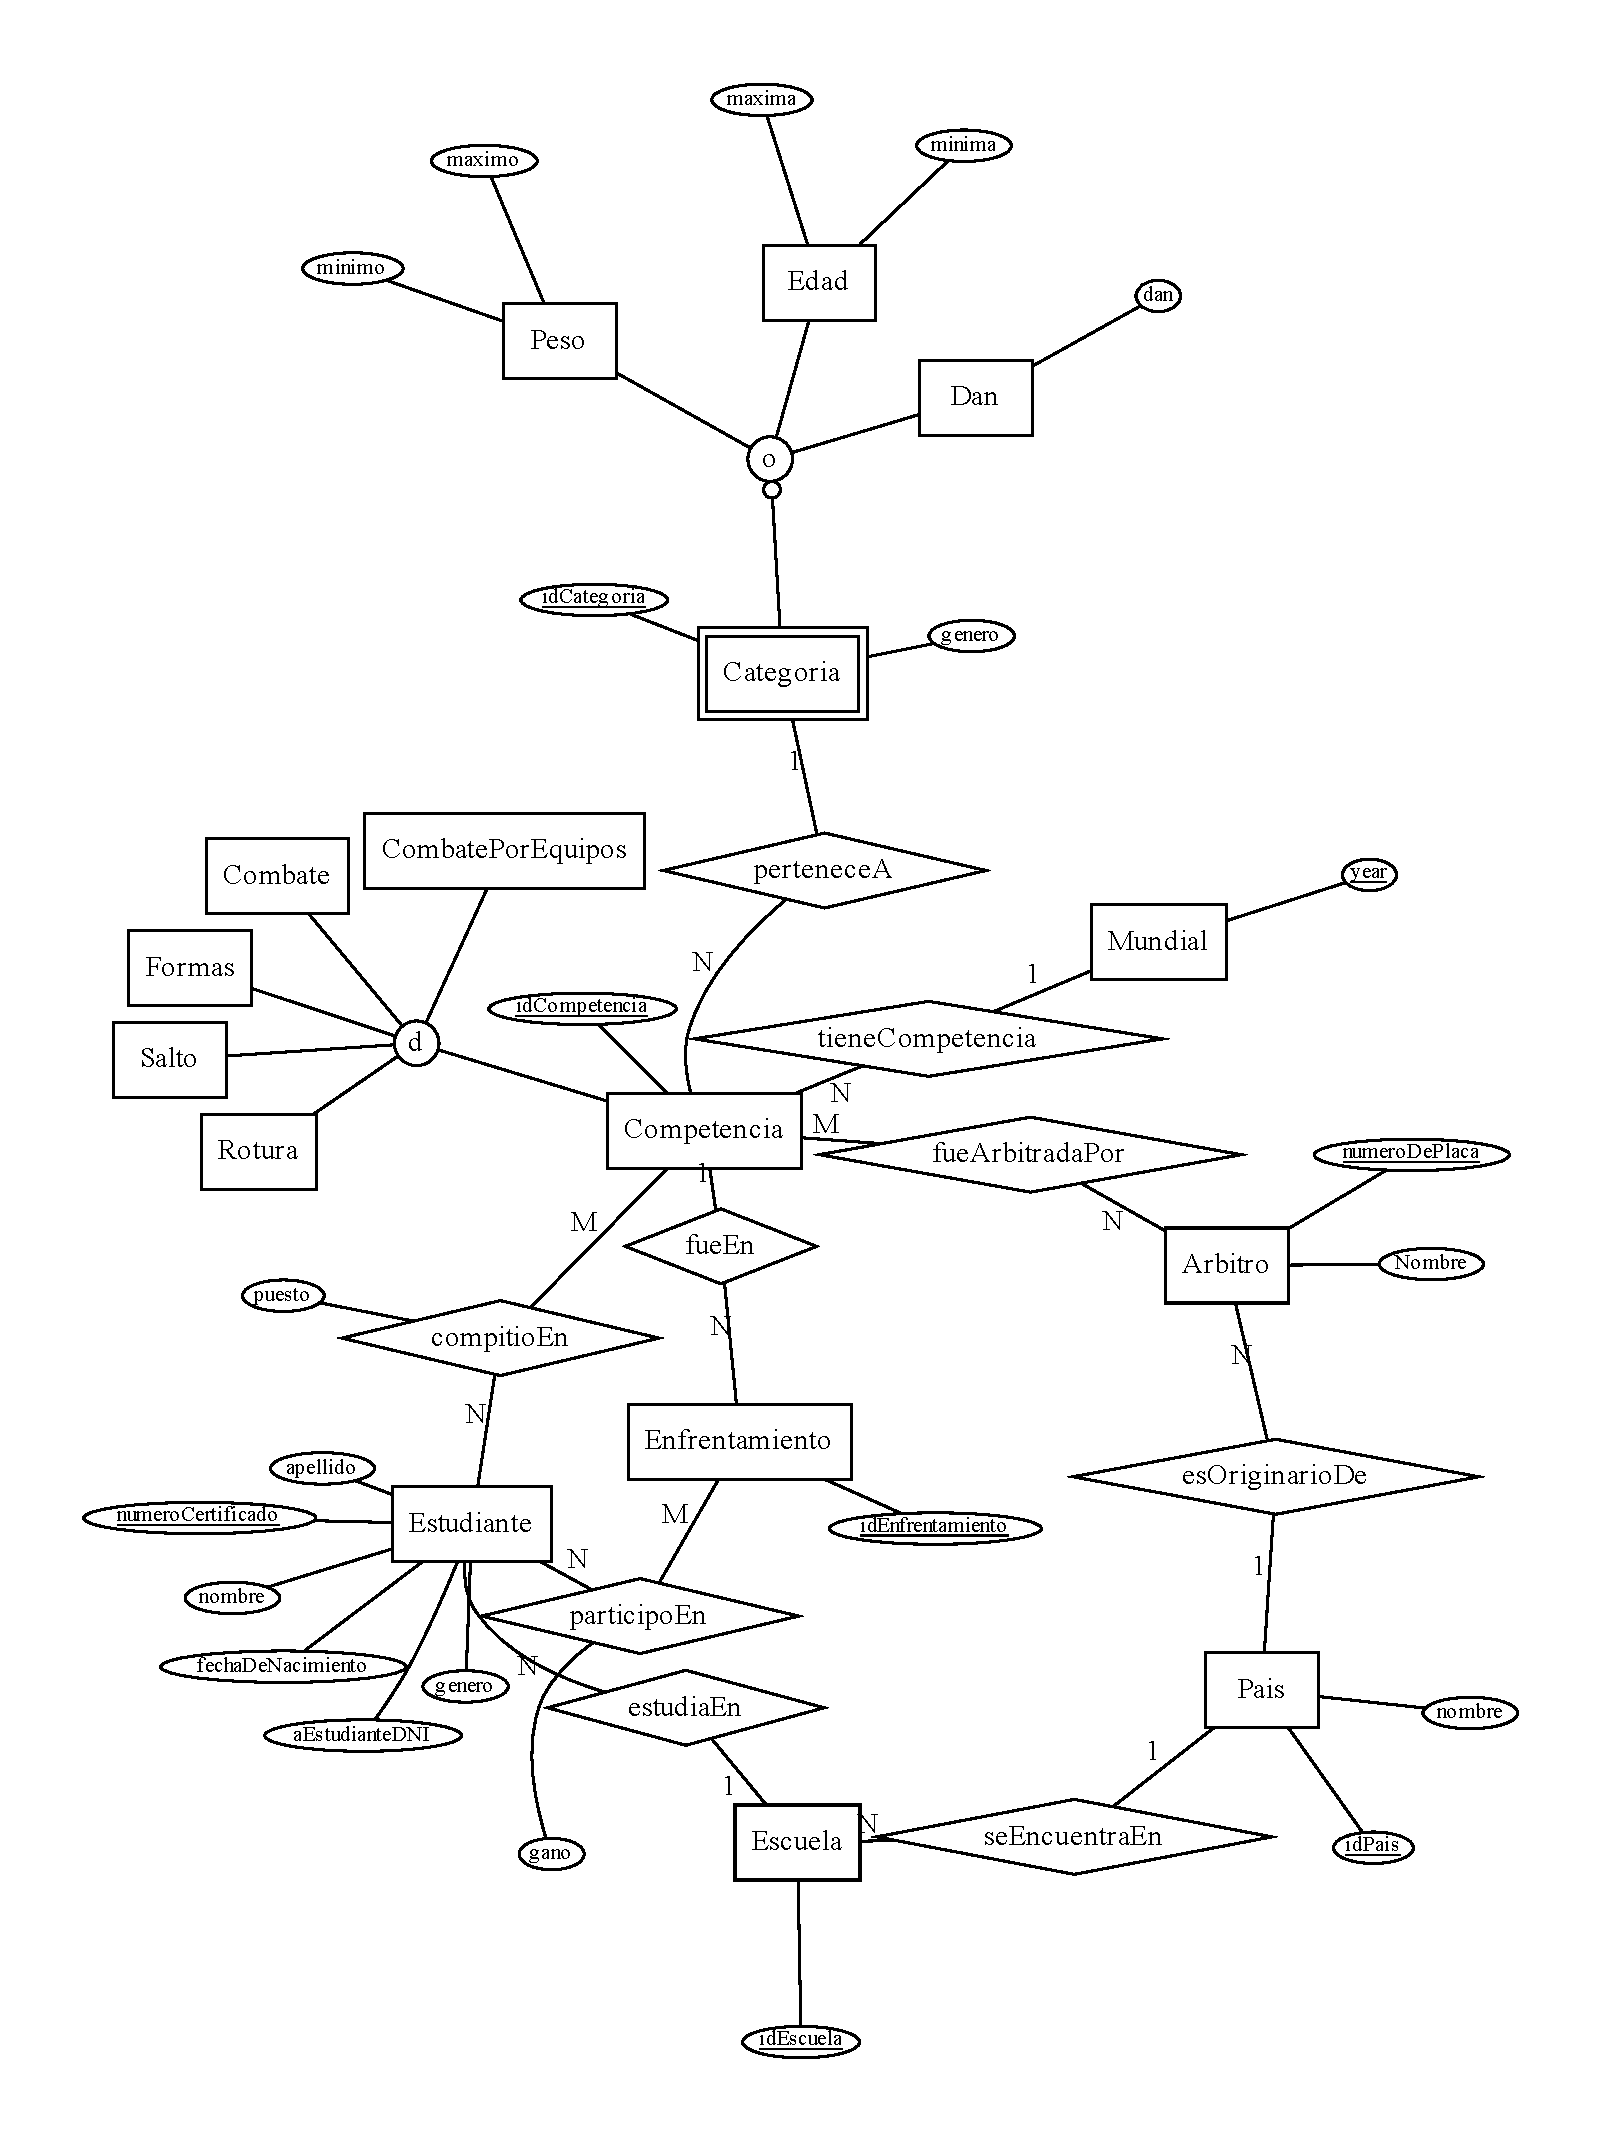
\includegraphics[width=\textwidth]{../mer/mer-neato.pdf}


\newpage

\subsection{Diagrama de Interacción de Documentos}
% https://drive.google.com/file/d/0B3FgdUXk8fTrNWUwQ0tpLWFsbE0/view?usp=sharing

\begin{figure}[H]
  \centering
  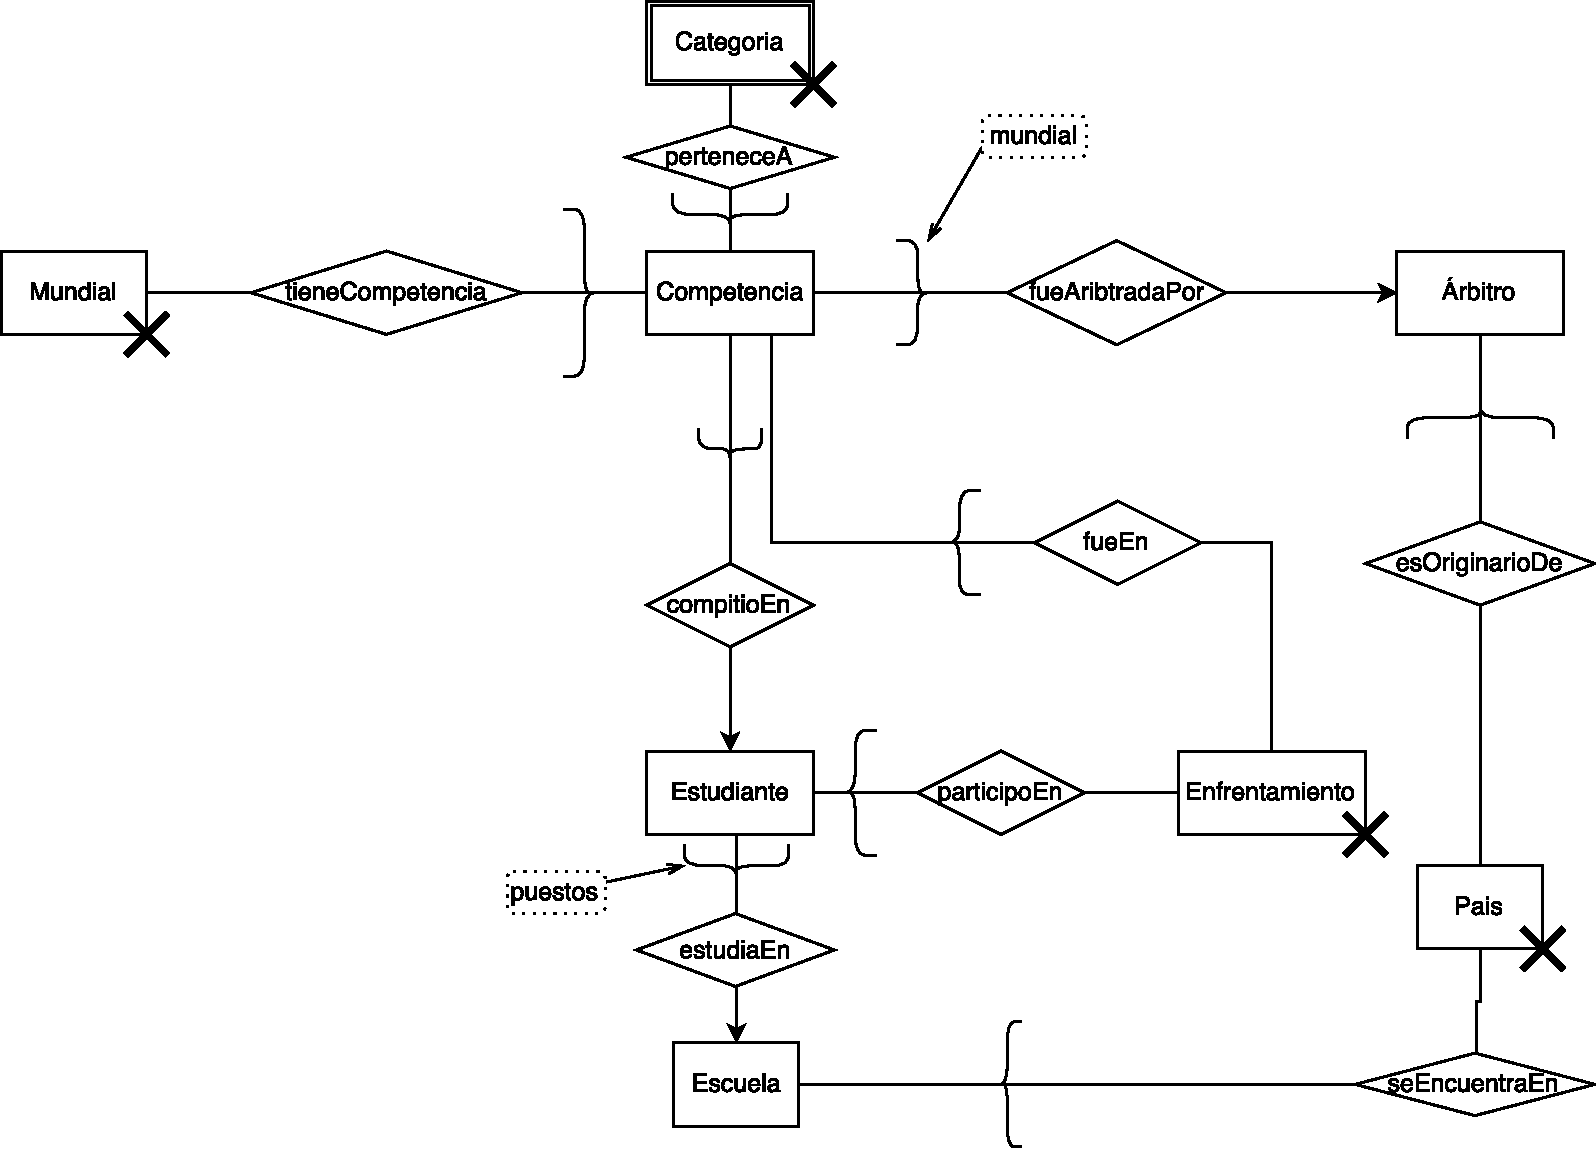
\includegraphics[width=\textwidth]{img/did.pdf}
  \caption{Diagrama de Interacción de Documentos. Se omiten atributos y cardinalidad de las relaciones por simplicidad, pero son las mismas que en el diagrama de entidad relación.}
\end{figure}

Notemos que las entidades que tendremos en nuestro json schema (y por lo tanto en nuestra base de datos) serán solamente cuatro: Competencia, Árbitro, Estudiante y Escuela.

Cuando embebemos entidades en otras lo hacemos sobre todo para poder cumplir con las queries y además hacerlo de manera eficiente.

Por ejemplo, embebemos los puestos de los estudiantes en escuela para poder hacer rápidamente la query 2.2 (\textit{La cantidad de medallas por nombre de escuela en toda la historia}).

Similarmente, embebemos el mundial de la competencia en Árbitro para poder realizar la query 2.4 (\textit{Los árbitros que participaron en al menos 4 campeonatos}) de manera eficiente.

La eliminación de las entidades País y Categoría es muy razonable. Eliminamos también Mundial porque no es particularmente necesaria para ninguna query y no vale la pena duplicar la información. Finalmente, eliminamos Enfrentamiento, porque es redundante tenerla (dado que embeberla en Estudiante y en Competencia nos da toda la información que eventualmente podramos necesitar).

\newpage


\subsection{JSON Schema}
JSON Schema para Estudiante.
\begin{lstlisting}[language=json]
{
"type": "object", "properties": {
    "Nombre": { "type": "string" },
    "Apellido": { "type": "string" },
    "nroCertificado": { "type": "integer" },
    "Genero": { "type": "string" },
    "DNI": { "type": "integer" },
    "CodigoEscuela" : { "type": "integer"},
    "ResultadosPorMundial" : { "type": "array", "items": {
        "Resultado": { "type": "object", "properties": {
            "Mundial": { "type": "object", "properties": {
                "Nombre": { "type": "string" },
                "Year": { "type": "integer" } } },
            "Competencias" : { "type" : "array", "items": {
                "Competencia": { "type": "object", "properties": {
                    "TipoCompetencia": { "type": "string" },
                    "Puesto": { "type": "integer" },
                    "Enfrentamientos": { "type": "array", "items": {
                        "Enfrentamiento": { "type": "object", "properties": {
                            "nroCertificadoDelOponente": { "type": "integer" },
                            "Gano": { "type" : "integer" } } } } } } } } } } } } } }
}
\end{lstlisting}

JSON Schema para Escuela.
\begin{lstlisting}[language=json]
{
"type": "object", "properties": {
    "Nombre": { "type": "string" },
    "pais": { "type": "string" },
    "CodigoEscuela": { "type": "integer" } },
    "Resultados": { "type" : "array", "items": {
        "Resultado": { "type": "object", "properties": {
            "Mundial": { "type": "object", "properties": {
                "Nombre": { "type": "string" },
                "Year": { "type": "integer" } } },
            "Puestos": { "type": "array", "items": { "type": "integer" } } } } } }
}
\end{lstlisting}

JSON Schema para Árbitro.
\begin{lstlisting}[language=json]
{
"type": "object", "properties": {
    "nroPlaca": { "type": "integer" },
    "Nombre": { "type": "string" },
    "pais": { "type": "string" },
    "Mundiales": { "type": "array", "items": {
        "Mundial": { "type": "object", "properties": {
            "Nombre": { "type": "string" },
            "Year": { "type": "integer" } } } } } }
}
\end{lstlisting}

JSON Schema para Competencia.
\begin{lstlisting}[language=json]
{
"type": "object", "properties": {
   "idCompetencia": { "type": "integer" },
   "Categoria": { "type": "object", "properties": {
       "idCategoria": { "type": "integer" },
       "Genero": { "type": "string" },
       "Dan": { "type": "integer" },
       "EdadMinima": { "type": "integer" },
       "EdadMaxima": { "type": "integer" },
       "pesoMinimo": { "type": "integer" },
       "pesoMaximo": { "type": "integer" } } },
    "TipoCompetencia": { "type": "string" },
    "Enfrentamientos": { "type": "array", "items": {
        "Enfrentamiento": { "type": "object", "properties": {
            "nroCertificadoPrimerCompetidor": { "type": "integer" },
            "nroCertificadoSegundoCompetidor": { "type": "integer" },
            "Gano": { "type" : "integer" } } } },
    "Puestos": { "type": "array", "items": {
        "ParticipantePuesto": { "type": "object", "properties": {
            "nroCertificado": { "type": "integer" },
            "puesto": { "type": "integer" }
        } } } },
    "Arbitros": { "type": "array", "items": {
        "nroDePlaca": "integer" } },
    "Mundial": { "type": "object", "properties": {
        "Nombre": { "type": "string" },
        "Year": { "type": "integer" } } } } }
}
\end{lstlisting}

\par Los Schemas presentados arriba se derivan del Diagrama de Interacción de Documentos, aunque con ciertas sutilezas.

\par A saber, Competencia se encuentra parcialmente embebida en Estudiante; sólo los Enfrentamientos y los Puestos que le corresponden a cada competidor se encuentran embebidos en su documento.
En el caso de los enfrentamientos, el número de certificado embebido es el del oponente.
A su vez, si bien Mundial se encuentra en Competencia, en ResultadosPorMundial los Resultados separan Mundial de 
todas las Competencias que se llevaron a cabo en éste.
Esto sería equivalente a embeber tradicionalmente y luego agrupar.
Se procedió de esta forma ya que es más eficiente tanto en términos de memoria como de velocidad y simplicidad de
las queries\footnote{Notar que se está representando exactamente lo estipulado por el DID, 
sólo agrupándolo de otra forma.}.

\par En Escuela se embeben parcialmente los Estudiantes, nuevamente de una forma similar: se separa el Mundial 
de los Puestos, para evitar repeticiones innecesarias y facilitar las queries.

\newpage

\section{RethinkDB}


RethinkDB es...


\subsection{Sharding}

La consigna del TP pide experimentar con sharding. Para esto utilizamos la tabla que contiene a todos los árbitros, dado que es la más fácil de generar valores aleatorios para insertar.

Inicializamos la tabla con 1 shard y \textasciitilde 100 valores.

\begin{figure}[H]
 \centering
 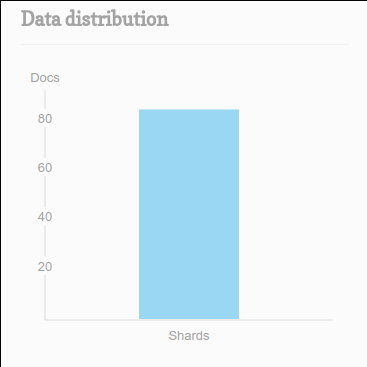
\includegraphics[width=2.5in]{sharding/img/1shard.png}
 \caption{1 shard con \textasciitilde 100 valores}
 \label{fig:1shard}
\end{figure}

Luego pasamos a 2 shards, manteniendo los \textasciitilde 100 valores.

\begin{figure}[H]
 \centering
 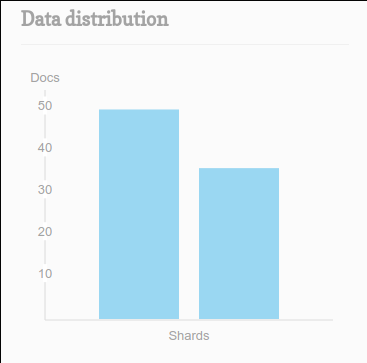
\includegraphics[width=2.5in]{sharding/img/2shard.png}
 \caption{2 shards con \textasciitilde 100 valores}
 \label{fig:2shard}
\end{figure}

Finalmente pasamos a 3 shards, manteniendo los \textasciitilde 100 valores.

\begin{figure}[H]
 \centering
 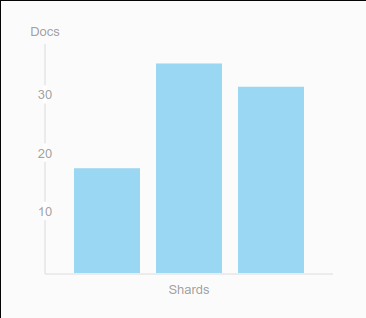
\includegraphics[width=2.5in]{sharding/img/3shard100.png}
 \caption{3 shards con \textasciitilde 100 valores}
 \label{fig:3shard100}
\end{figure}

Luego empezamos a aumentar la cantidad de documentos de la tabla, de a cientos o a más. Graficamos las siguientes cantidades: 100, 200, 300, 400, 700, 1000, 1500, 2000, 4000. Se puede apreciar que la distrubución que vemos cuando hay sólo 100 documentos perdura a lo largo de todas las inserciones.

\begin{figure}[H]
\centering
\begin{tabular}{|l | l | l | l|}
  \hline
  \# Documentos & Shard 1 & Shard 2 & Shard 3 \\
  \hline
  100           & 18  & 36  & 32 \\
  200           & 50  & 80  & 70 \\
  300           & 65  & 115 & 95 \\
  400           & 84  & 170 & 115 \\
  700           & 145 & 265 & 235 \\
  1000          & 185 & 395 & 306 \\
  1500          & 265 & 563 & 480 \\
  2000          & 405 & 747 & 700 \\
  4000          & 718 & 1595 & 1384 \\
  \hline
\end{tabular}
 \caption{Tabla de como avanza la distribución de documentos por shard cuando insertamos más documentos. Notar que todos los valores, que fueron extraídos de la interfaz gráfica de RethinkDB, son aproximados, RethinkDB no garantiza exactitud en estas estadísticas.}
 \label{fig:shardstabla}
\end{figure}


\begin{figure}[H]
 \centering
 \includegraphics[width=5in]{shards.pdf}
 \caption{Gráfico de la tabla anterior}
 \label{fig:shardslinea}
\end{figure}


Por ejemplo, veamos la distribución con \textasciitilde 4000 documentos:
\begin{figure}[H]
 \centering
 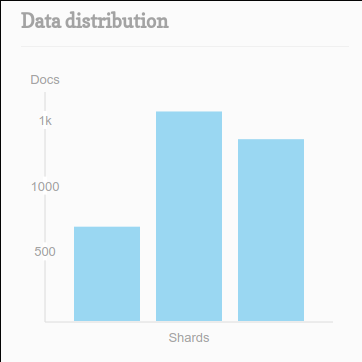
\includegraphics[width=2.5in]{sharding/img/3shard4000.png}
 \caption{3 shards con \textasciitilde 4000 valores}
 \label{fig:3shard4000}
\end{figure}

\newpage
\subsection{Consultas}

\emph{La cantidad de enfrentamientos ganados por competidor para un campeonato dado.}\footnote{La query 
se muestra con los placeholders nroCert y yearMund para el número de certificado y el año del campeonato, 
respectivamente.}
\begin{lstlisting}[language=rethinkDBnoSQL]
r.db("TP2").table("estudiante").get(nroCert).
getField("ResultadosPorMundial").filter(
{"Mundial": {"Year": yearMund}}).nth(0).
getField("Competencias").concatMap(function (val) 
  { return val.getField("Enfrentamientos").filter({"Gano": 1})});
\end{lstlisting}

\emph{La cantidad de medallas por nombre de escuela en toda la historia.}
\begin{lstlisting}[language=rethinkDBnoSQL]
r.db("TP2").table("escuela").map(function(x) { return {"Nombre": x.getField("Nombre"), "Medallas":
  x.getField("Resultados").fold(0, function (b, y) 
    { return y.getField("Puestos").filter(function(z) { return z.lt(4)}).count().add(b)})}});
\end{lstlisting}

\emph{Para cada escuela, el campeonato donde ganó más medallas.}
\begin{lstlisting}[language=rethinkDBnoSQL]
r.db("TP2").table("escuela").map(function(x) { return {"Nombre": x.getField("Nombre"), 
  "MundialDondeMasGano":
  x.getField("Resultados").reduce(function (b, y) 
    { return r.branch(y.getField("Puestos").filter(function(z) { return z.lt(4)}).count().gt(
      b.getField("Puestos").filter(function(z) { return z.lt(4)}).count()), y, b)}).getField("Mundial")}});
\end{lstlisting}

\emph{Los árbitros que participaron en al menos 4 campeonatos.}
\begin{lstlisting}[language=rethinkDBnoSQL]
r.db("TP2").table("arbitro").filter(function (x) { return x.getField("Mundiales").count().gt(3) });
\end{lstlisting}

\emph{Las escuelas que han presentado el mayor número de competidores en cada campeonato.}
\begin{lstlisting}[language=rethinkDBnoSQL]
r.db("TP2").table("escuela").concatMap(function(x){return
  x.getField("Resultados").map(function(y){return {"Nombre": x.getField("Nombre"),
    "YearMundial": y.getField("Mundial").getField("Year"), 
    "NroCompetidores": y.getField("Puestos").count()}})}).group("YearMundial").
  reduce(function (b, w) 
    {return r.branch(w.getField("NroCompetidores").gt(
      b.getField("NroCompetidores")), w, b)});
\end{lstlisting}

\emph{Obtener los competidores que más medallas obtuvieron por modalidad.}
\begin{lstlisting}[language=rethinkDBnoSQL]
r.db("TP2").table("estudiante").map(function(x){ return {"Nombre": x.getField("Nombre"), 
  "CantidadDeMedallasPorModalidad": x.
  getField("ResultadosPorMundial").concatMap(function(y){
    return y.getField("Competencias")}).filter(function(w){
    return w.getField("Puesto").lt(4)}).pluck("TipoCompetencia").
  group("TipoCompetencia").count().ungroup()}}).
  filter(function(x){ return r.not(x.getField("CantidadDeMedallasPorModalidad").isEmpty())}).
  map(function(x){ return {"Modalidad": x.getField("CantidadDeMedallasPorModalidad").
    getField("group").nth(0), "CantidadDeMedallas": x.getField("CantidadDeMedallasPorModalidad").
    getField("reduction").nth(0), "Nombre": x.getField("Nombre")}}).
  group("Modalidad").max("CantidadDeMedallas");
\end{lstlisting}

Notar que las últimas dos queries fueron implementadas utilizando Map-Reduce.


\section{Conclusión}
\par Al emplear embedding de Competencia en Estudiante y a la vez de éste en Escuela, agrupando los datos 
por Mundial, logramos queries eficientes que requieren un único acceso a tabla, con cierta pero no excesiva 
redundancia\footnote{Notar que si se quisiera priorizar la eficiencia de memoria, 
Competencia se podría transformar en una entidad débil y se podrían seguir llevando
a cabo las queries pautadas.}.

\par Para ciertas queries\footnote{En particular, las dos últimas.}, el método Map-Reduce nos resultó ideal.

\newpage


%\begin{thebibliography}{9}
%
%\bibitem{inpractice}
%  Len Bass et al.,
%  \emph{Software Architecture in Pratice}.
%  Addison-Wesley,
%  2nd edition.
%
%\end{thebibliography}


\end{document}
